%
% Appendix A
%

\chapter{SVFit Mass}
\label{SVFit}

A study has been performed to improve the next iteration of the search for LFV decays of the Higgs boson. In this study, we have observed that using the ``Classic'' SVFit (Sensitivity Volume Fit) algorithm can help improve the signal resolution compared to the collinear mass resolution~\cite{Bianchini:2016yrt}. The ``Classic'' SVFit algorithm has been developed to reconstruct the mass of a Higgs boson decaying into two tau leptons \mtt and is an improved version of the SVFit algorithm. The SVfit algorithm~\cite{Bianchini:2014vza} has been used to reconstruct the Higgs boson mass in the SM \Htt analysis and searches for further Higgs bosons predicted by models beyond the SM performed by the CMS collaboration during LHC Run 1. Compared to alternative mass variables, the SVfit algorithm's usage has improved the SM \Htt analysis's sensitivity for measuring the signal rate by $\approx 40\%$~\cite{Chatrchyan:2014nva}. The improvement in sensitivity corresponds to a gain by about a factor of two in the integrated luminosity of the analyzed dataset.

The ``Classic'' SVFit algorithm uses a likelihood function of arbitrary normalization. The algorithm allows for the reconstruction of not only the mass \mtt of the tau lepton pair but any kinematic function of the two tau leptons, including the \pt, $\eta$, and $\phi$ and transverse mass of the tau lepton pair. A further improvement concerns the algorithm's extension to account for the experimental resolution on the reconstruction of hadrons produced in the tau decays. The ``Classic'' SVFit algorithm was modified to reconstruct the mass of the Higgs boson decaying into LFV decay modes \mlt. A brief description of the algorithm is given in the following paragraphs.

\section{``Classic'' SVfit algorithm}
As only one of the lepton from an LFV Higgs decay is a tau, it was modified so that the matrix element of the probability density function defined can reconstruct the Higgs mass \mlt. The phase space of the tau decay products along with the angles $\theta_{inv}$ and $\phi_{inv}$ are illustrated in Figure~\ref{fig:sv}. The $\bp_{inv}$ vector is located on the surface of a cone, the axis of which is given by the $\bp_{vis}$ vector. The variable $\phi_{inv}$ represents the angle of rotation, in a counter-clockwise direction, around the cone's axis. The value $\phi_{inv} = 0$ is chosen to correspond to the case that the $\bp_{inv}$ vector is within the plane spanned by the $\bp_{vis}$ vector and the beam direction.

\begin{equation}
  \begin{aligned}
    \mathcal{L}\left(\bp^{\text{vis}} ; p_{\text{x}}^{\text{rec}}, p_{\text{y}}^{\text{rec}} \mid \mh \right)=\frac{32 \pi^{4}}{s} \int \text{d} \mh \text{d} \Phi_{n} \left|\text{BW}_{\Pgt}\right|^{2} \left|\mathcal{M}_{\Pgt \rightarrow \ldots}(\tilde{\bp})\right|^{2} \\
    W\left(\bp^{\text{vis}} \mid \hat{\bp}^{\text{vis}}\right) W_{\text{rec}}\left(p_{\text{x}}^{\text{rec}}, p_{\text{y}}^{\text{rec}} \mid \hat{p}_{\text{x}}^{\text{rec}}, \hat{p}_{\text{y}}^{\text{rec}} \right) \mathcal{F}(\bp)
  \end{aligned}
\end{equation}

\begin{figure*}[!htpb]
  \centering
  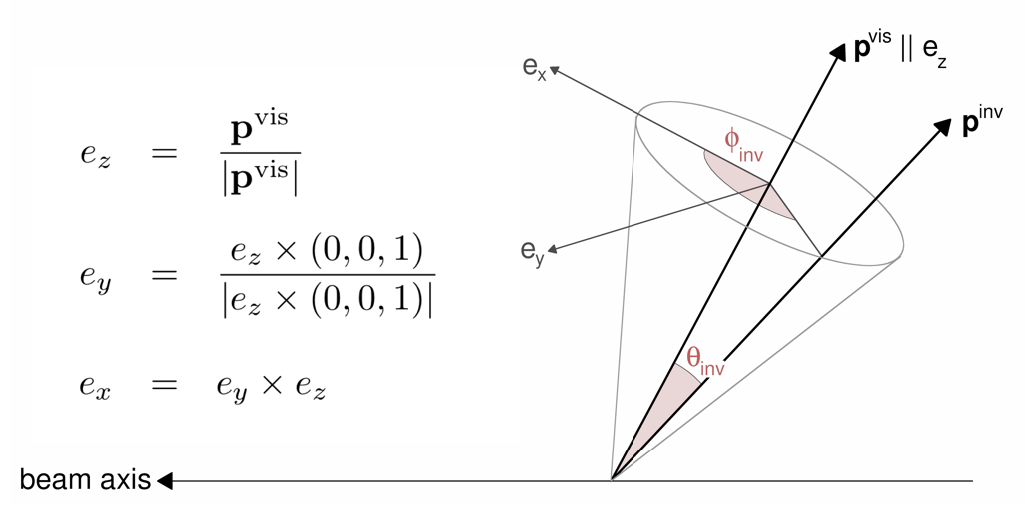
\includegraphics[width=0.9\textwidth]{plots/appendix/SV.png}
  \caption{Illustration of the variables $\theta_{inv}$ and $\phi_{inv}$ that specify the orientation of the $\bp_{inv}$ vector relative to the momentum vector $\bp_{vis}$ of the visible tau decay products.}
  \label{fig:sv}
\end{figure*}

The function $\mathcal{F}(\bp)$ in the integrand may be an arbitrary function of the momenta of the prompt and tau leptons. The integral is evaluated numerically, using a custom implementation of the Markov chain MC integration method with the Metropolis-Hastings algorithm~\cite{Hastings:1970aa}. The actual value $\mathcal{L}(y)$ of the integral is irrelevant. The reconstruction of the mass \mlt of the prompt and tau lepton pair is based on choosing:
%
$\mathcal{F}(\bp) \equiv \left(\hat{E}_{\ell} + \hat{E}_{\Pgt}\right)^{2} - \left(\left(\hat{p}_{\text{x}}^{\ell}+\hat{p}_{\text{x}}^{\Pgt}\right)^{2}+\left(\hat{p}_{\text{y}}^{\ell}+\hat{p}_{\text{y}}^{\Pgt}\right)^{2}+\left(\hat{p}_{\text{z}}^{\ell}+\hat{p}_{\text{z}}^{\Pgt}\right)^{2}\right)$,
%
recording the values of $\mathcal{F}(\bp)$ for each evaluation of the integrand by the Markov chain and taking the median of the series of $\mathcal{F}(\bp)$ values as the best estimate \mlt for the mass of the prompt and tau lepton pair in a given event. The total number of evaluations of the integrand referred to as Markov chain ``states'', amounts to 100000 per event. The first 10000 evaluations of the integrand are used as a ``burn-in'' period and are excluded from the median's computation.

Figure~\ref{fig:svfit} shows the collinear mass and SVFit mass distributions. The distributions are fit with a double Gaussian, and the goodness of fit as tested from $\chi^2/\text{ndof}$ is close to one, suggesting that it is a good fit. The full width at half maximum is used for inferring the signal resolution, and it has a value of 38.88~\GeV for collinear mass, while for SVFit mass, the value is 30.90~\GeV. This corresponds to a 20\% improvement in signal resolution. The collinear mass and SVFit mass are peaking close to the Higgs mass of 125~\GeV. The collinear mass has a higher mean of $\sim 129 \GeV$ due to its larger tail, while SVFit mass has a mean of $\sim 117 \GeV$ due to it's smaller tail distribution.

\begin{figure*}[!htpb]
  \centering
  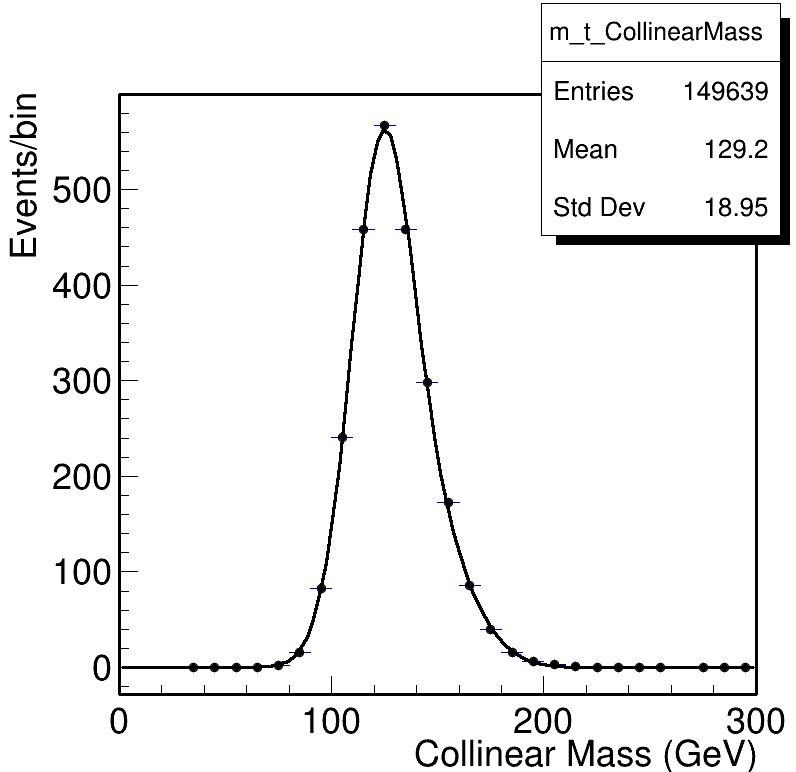
\includegraphics[width=0.45\textwidth]{plots/appendix/CollMass.png}
  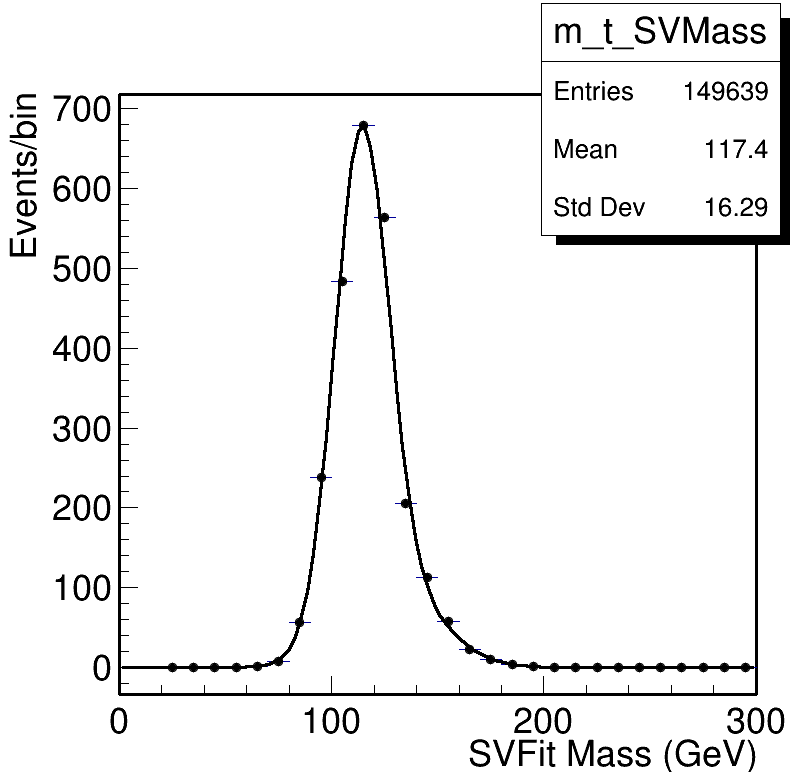
\includegraphics[width=0.45\textwidth]{plots/appendix/SVFit.png}
  \caption{Collinear mass vs SVFit mass.}
  \label{fig:svfit}
\end{figure*}

This study has shown that mass resolution is significantly improved by using the SVFit mass instead of the collinear mass, and it can give much more sensitive results for the \Hmt and \Het searches. A future search using the full Run 3 data can benefit from this improved sensitivity, and the SVFit can easily be extended to be used for heavy Higgs boson searches. The only disadvantage that was noted during the study was from the computing point of view. It takes an order of magnitude longer time to compute the SVFit mass than the collinear mass, which has to be investigated and improved in any future analysis.
